\problemname{Dansk}

\noindent
Boschua skal flytte til Lund for at studere ved LTH. 
Du har fundet ud af, at Lund ligger i Skåne, og nu er du bekymret for, at Boschua begynder at lyde dansk.

For at forhindre dette vil du vise Boschua, hvor mange ord der overhovedet ikke lyder danske. 
Ifølge dig lyder et ord dansk, hvis det indeholder mindst ét ord fra den danske ordbog. 
Desværre ejer du ikke den officielle danske ordbog, men den gamle ordbog, du fandt i kælderen, må gøre det.

For eksempel, antag at ordbogen kun indeholder ordet \texttt{knallert}. Så mener du, at ordet \texttt{hus\textbf{knallert}rumma} 
lyder dansk, fordi det indeholder ordet \texttt{knallert}. Derimod mener du, at ordet \texttt{\textbf{knaller}un\textbf{t}} \textbf{ikke} 
lyder dansk, fordi det ikke indeholder \texttt{knallert}.

\begin{figure}[h]
  \centering
  \begin{minipage}{0.45\textwidth}
    \centering
    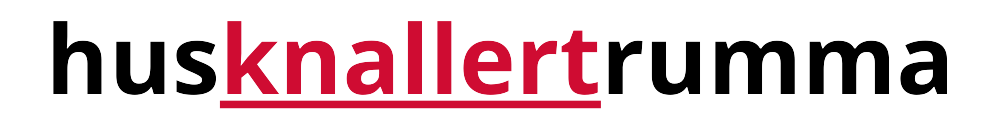
\includegraphics[scale=0.7]{danska-knallert.png}
    \caption{Ordet \texttt{husknallertrumma} lyder dansk.}
  \end{minipage}\hfill
  \begin{minipage}{0.45\textwidth}
    \centering
    
\includegraphics[scale=0.7]{knallerunt.png}
    \caption{Ordet \texttt{knallerunt} lyder ikke dansk.}
  \end{minipage}
\end{figure}

Du indser hurtigt, at der er for mange ord, der ikke lyder danske, til at skrive dem alle ned. 
Derfor tænker du, at det er nok at tælle antallet af ord, der ikke lyder danske, og fortælle det til Boschua. 
Selv dette viser sig at være svært, fordi der er så mange ord, der ikke lyder danske.

Til sidst nøjes du med at tælle antallet af ord, der kun består af små engelske bogstaver 
\texttt{a}-\texttt{z}, har præcis $N$ bogstaver, og ikke lyder danske. Et ord lyder for dansk, hvis det indeholder 
mindst ét ord fra ordbogen som en delstreng.

\section*{Input}
Den første linje i inputtet indeholder heltallene $N$ ($1 \leq N \leq 100$) og $M$ ($0 \leq M \leq 150$), 
længden af de ord, vi betragter, og antallet af ord i ordbogen.

Derefter følger $M$ linjer, hvor hver linje indeholder et ord fra ordbogen. Alle disse ord har en længde på højst $N$ 
og består af bogstaverne \texttt{a}-\texttt{z}. Alle disse ord er desuden unikke.

\section*{Output}
Udskriv antallet af ord med længde $N$, der ikke lyder for danske. Da dette tal kan blive meget stort, 
udskriv det \href{https://en.wikipedia.org/wiki/Modulo}{modulo} $10^9+7$. 

\section*{Pointsystem}
Din løsning vil blive testet på en række testgrupper, hver med en vist antal point. 
Hver testgruppe indeholder en række testfald. For at opnå point for en testgruppe skal du løse alle testfald i testgruppen. 

\noindent
\begin{tabular}{| l | l | p{12cm} |}
  \hline
  \textbf{Gruppe} & \textbf{Point} & \textbf{Begrænsninger} \\ \hline
  $1$    & $10$       & $M = 0$ \\ \hline
  $2$    & $13$       & $N \leq 3, M \leq 10$ \\ \hline
  $3$    & $23$       & $M = 1$ \\ \hline
  $4$    & $32$       & $N, M \leq 50$ \\ \hline
  $5$    & $22$       & Ingen yderligere begrænsninger. \\ \hline
\end{tabular}

\section*{Forklaring af eksempler}
I det første tilfælde findes der $26^3$ forskellige ord. Da den danske ordbog er tom i dette tilfælde, forbydes ingen af dem.
